\documentclass{article}
\setlength{\parindent}{0cm}

@(vfl) = **Vanilla Flavored LaTex**

@(github_url) = http://github.com/adhithyan15/vanilla

@(tmaker) = **TexMaker**

@(ftb) = formatted text blocks

#(cftb)[] = [$(capitalize)[formatted text blocks]]

$(importpack)[documentation]

\begin{document}

\begin{center}

\huge{Vanilla Documentation}\vspace{5pt}

\large{**Adhithya Rajasekaran**}

\end{center}

\vspace{30pt}

\section*{What is Vanilla?}

Vanilla is a powerful LaTex preprocessor. It works based on the DRY(Don't Repeat Yourself) principle. It aims to reduce the entry barrier and learning curve for Latex by simplifying the syntax and also reducing the verbosity of Latex. In this documentation you will learn how to write Vanilla flavoured Latex documents. This document itself is written in Vanilla flavoured Latex. \vspace{5pt}

Let us start off with why I created Vanilla. \vspace{5pt}

\section*{Why Vanilla?}

I was trying to teach my mom, who is a high school math teacher, to use Latex. I was unsuccessful in that endeavour because my mom found Latex syntax very verbose and she hated the steep learning curve of Latex. I started to wonder if there are any ways to reduce the learning curve of Latex and also reduce the verbosity of Latex. I stumbled across \textbf{Markdown}, a small markup language that compiled into HTML. The syntax of Markdown was very intuitive and short. So I decided to implement a lot of ideas from Markdown into Latex and that's how Vanilla was born. 

\section*{Technical Details}

Vanilla first started out as a separate markup language with backward compatiblity to Latex. But I dropped that idea and made it as an extension of Latex so that people can keep using their editors. Vanilla compiler prototype was written in Python. Then the code was translated into Ruby and was released as a command line utility.

\section*{Getting Vanilla}

It is very easy to get Vanilla. Visit www.adhithyan15.github.com/vanilla/ and follow the steps below. 

\begin{enumerate}

\item Click on ``Download Zip'' to download both the source of the compiler and also the compiled version of the compiler. \vspace{5pt}

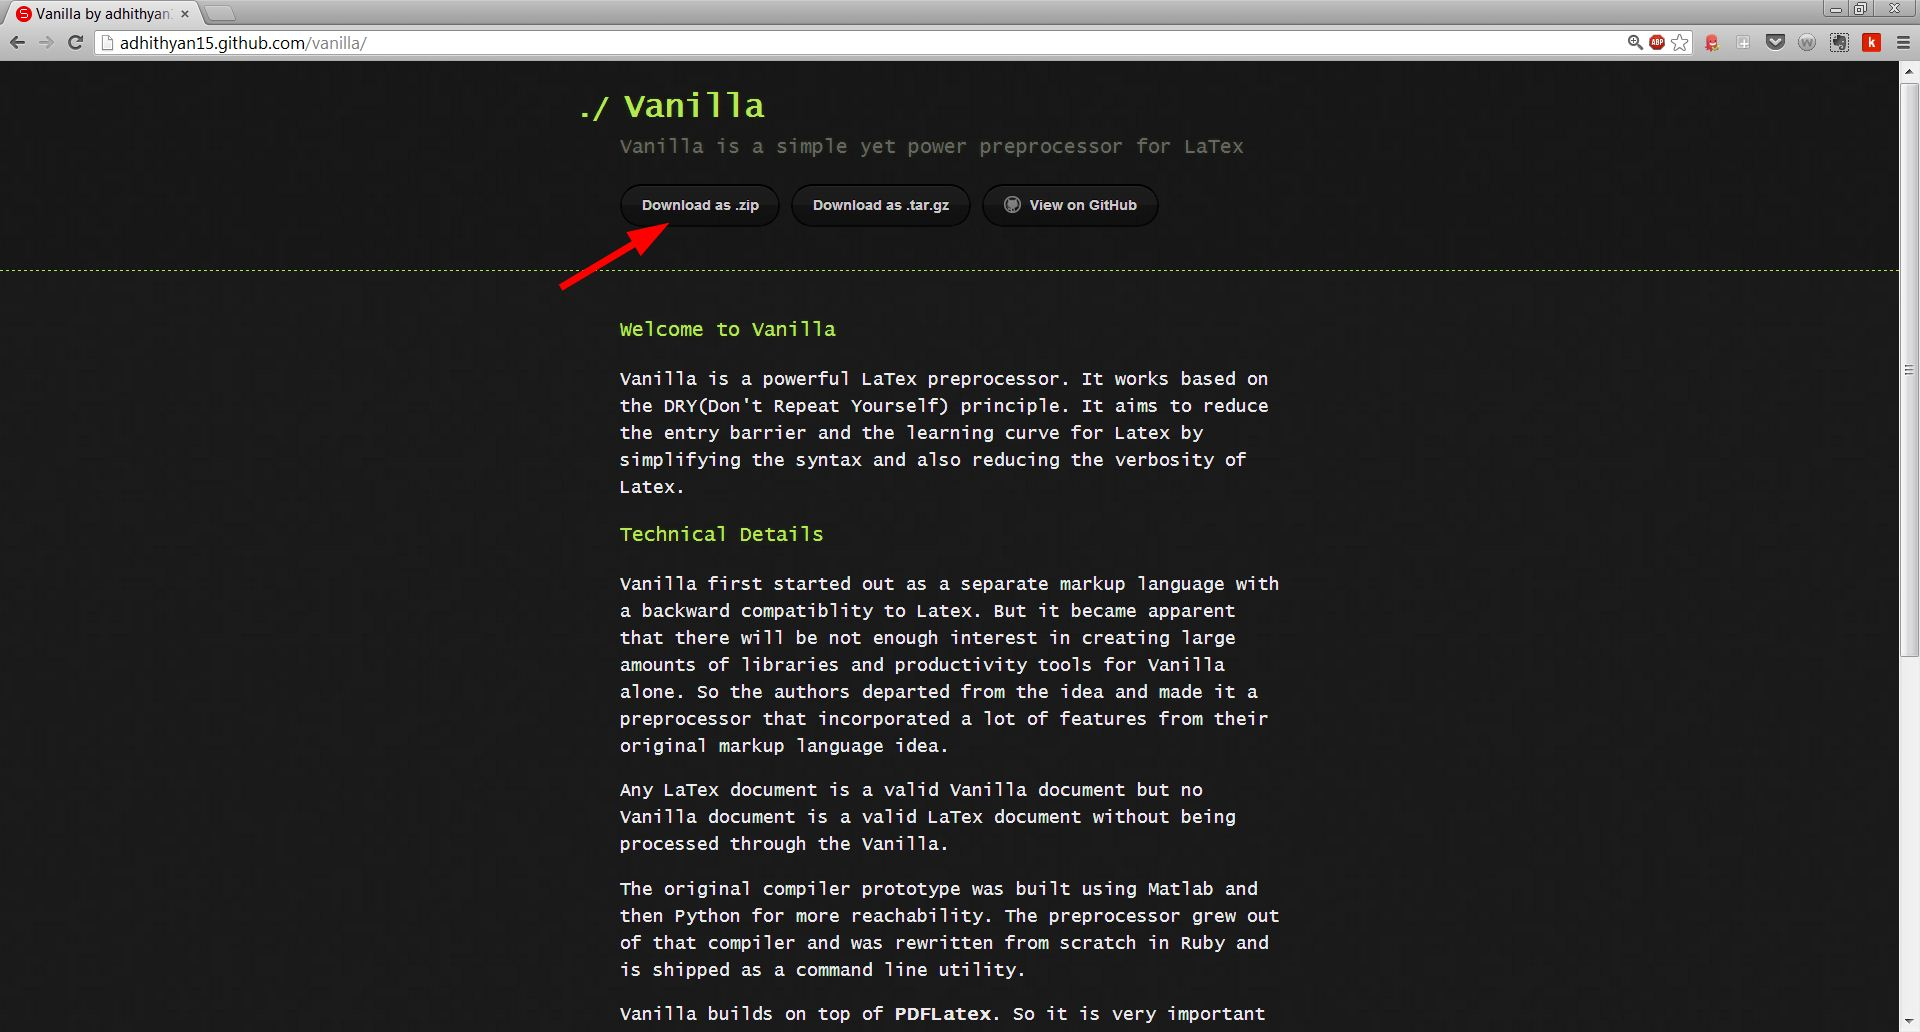
\includegraphics[scale=0.5]{VanillaGithub}

\item Extract the downloaded zip file using Winzip or any other archive extractor. If you don't have an archive extractor, I recommend *[ 7-zip => www.7zip.org ]

\item Once you extract it, you will find the following files inside the folder you extracted

\begin{itemize}

\item Vanilla.exe  -> This is the primary compiler that will help you compile @(vfl) to **Pure LaTex**. This might be of no use to you if you are running linux or mac. 
\item Vanilla.rb  ->  This file contains the source code of the compiler. If you are in mac or linux, you can use this file to compile your **Vanilla Flavored LaTex** to LaTex documents.
\item Readme.md ->  Since the project is hosted in *[ Github => @(github_url) ], Github added a readme file markuped in **Markdown**.
\item Documentation.pdf ->  This is the same document that you are reading right now. 
\item Documentation.tex ->  This is the .tex version of documentation written using @(vfl). I highly recommend you to read through this document so that you can get example usages of @(vfl). 

\end{itemize}

%{4. If you don't have a LaTex editor, I highly recommend *[ TexMaker => http://www.xm1math.net/texmaker/]. It is the best LaTex editor that I was able to find. In the next section, we will learn how to configure **TexMaker** to use @(vfl).}%
 
\end{enumerate}

Vanilla compiler can work with LaTex Editors. But I request you to not use it because there are some issues which are being worked out. I expect to resolve all the issues by Version 2.0. So please wait until such time.

\section*{Features of Vanilla}

@(vfl) offers a lot of features to enhance people's productivity with LaTex. Let us see what those features below

\begin{itemize}

\item **Multiline Comments**: In @(vfl) you can comment out multiple lines of code using matlab style comments. Let us see a quick demo of this feature

###

%Vanilla Way

%You can comment out multiple lines using matlab style comments %{.....}%

%{Lorem ipsum dolor sit amet, consectetur adipiscing elit. Mauris placerat tristique purus, 
non tempus mi ultrices in. Praesent lobortis erat et lorem commodo mollis. Pellentesque 
eu euismod nulla.Ut vitae consequat est. Quisque adipiscing rhoncus tellus, eu fermentum 
augue tincidunt ut. Proin a dui dignissim massa auctor iaculis dictum a purus. Suspendisse 
porta felis at velit placerat varius.}%

###

Vanilla compiler converts @(vfl) multiline comments into several single line LaTex comments. Vanilla compiler doesn't touch the LaTex comments. So they are still valid. 

\item **Constants**: Constants are very similar to variables but they are immutable. In @(vfl), you can declare constants
through the following sytax $@(constant\_name) = value$. Note: LaTex has offers mutable variables. We are working on implementing mutable variables in Vanilla. It will be released in
version 2.0. 

###

%Vanilla way

%Vanilla forces you to declare your constants in your preamble so that it will 
%increase code readability. 

@(vfl) = **Vanilla Flavored LaTex** %must be declared in the preamble

%Usage

Welcome to @(vfl) %should output Welcome to \textbf{Vanilla Flavored LaTex} 

###

Vanilla compiler doesn't compile the Vanilla constants into LaTex variables. Instead, it converts them into plain text so that they can be used in a variety of purposes.  
Since the constants are rendered into plain text all the you can pass in a variable to most of the features listed below. 

\item **Formatted Text Blocks**: #(cftb)[] were inspired by Less CSS' parametric mixins. #(cftb)[] can include any kind of LaTex or @(vfl) formatting. 
@(vfl) forces the @(ftb) to be declared inside preamble to increase readability and @(ftb) are immutable. Mutable @(ftb) are under development and they will be released in version 2.0. 

###

%Declaration

#(welcome_message)[@(name),@(message)] = [Welcome **@(name)**,@(message)] %should be 
%declared in the preamble

%Usage

#(welcome_message)[Adhithya Rajasekaran,Hello World] %This should output 
%Welcome \textbf{Adhithya Rajasekaran}, Hello World

###

#(cftb)[] can span multiple lines. Parameterless @(ftb) can be used as a constants spanning multiple lines. 

###

%Declaration

#(disclaimer_statement)[] = [**WARNING**: Computer viruses can be transmitted via email. 
The recipient should check this email and any attachments for the presence of viruses. 
The company accepts no liability for any damage caused by any virus transmitted by this email.
E-mail transmission cannot be guaranteed to be secure or error-free as information could be 
intercepted, corrupted, lost, destroyed, arrive late or incomplete, or contain viruses. 
The sender therefore does not accept liability for any errors or omissions in the 
contents of this message, which arise as a result of e-mail transmission.] 
%must be declared in the preamble

%Usage

#(disclaimer_statement)[] %anywhere in the body

###

\item **Formulas**: Formulas were inspired by *[ Homebrew's => http://www.mxcl.github.com/homebrew/] formulas. @(vfl) is shipped with very few formulas
and the number is slowly increasing. The formulas that are shipped with @(vfl) are written for tasks that are difficult to do with LaTex. All the formulas will accept
accept a variable as a parameter. Let us take a look into the formulas that ship with @(vfl)

\begin{enumerate}

\item **Matrix Formula**: Matrices are very hard to construct in LaTex even with **AMSMATH** package. So @(vfl) ships with a -%\$(matrix)[]-% formula that allows
for the easy creation of matrices. This formula will create a matrix with square brackets around it.Let us do an example 

I want to create a matrix \vspace{5pt}

A = $(matrix)[1 2 3;4 5 6;7 8 9]

###

%using AMSMATH package

A = $\begin{bmatrix} 1 & 2 & 3 \\\\ 4 & 5 & 6 \\\\ 7 & 8 & 9 \end{bmatrix}$

%using Vanilla formula $(matrix)[]

A = $(matrix)[1 2 3;4 5 6;7 8 9]

###  

@(vfl) compiled the -%\$(matrix)[]-% formula into AMSMATH's **bmatrix** environment. 

\item **Determinant Formula**: Determinants are very similar to matrices except they use a straight line to enclose the contents of the matrix. @(vfl) ships with
the -%\$(det)[]-% formula that takes care of determinants. Let us see a quick demo of this feature

I want to create a determinant \vspace{5pt}

B = $(det)[1 2 3;4 5 6;7 8 9] 

###

%using AMSMATH package

B = $\begin{vmatrix} 1 & 2 & 3 \\\\ 4 & 5 & 6 \\\\ 7 & 8 & 9 \end{vmatrix}$

%using Vanilla formula $(matrix)[]

B = $(det)[1 2 3;4 5 6;7 8 9]

###

@(vfl) compiled the -%\$(det)[]-% formula into AMSMATH's **vmatrix** environment.

\item **Capitalize Formula**: Capitalize is a fun formula that capitalizes the first letter of every word in a string that is passed to it. Let us see a demo of this feature

###

$(capitalize)[this is a wonderful day] will yield This Is A Wonderful Day 

###

\end{enumerate}

As you can see that the number of formulas are very limited. Version 2.0 will allow users to create their own formulas using Ruby. 

\item **Inline Calculations**: Inline calculations allow you to perform simple yet powerful calculations with in the document. You can have to nest your calculations inside \#[] 
to perform the calculations. Let us see some examples

\begin{enumerate}

\item **-%![5*(45*(60/2))+3]-%** compiles into **![5*(45*(60/2))+3]**.

\end{enumerate}

\end{itemize}

\end{document}